% XeLaTeX

\documentclass{article}
\usepackage{ctex}
\usepackage{xypic}
\usepackage{amsfonts,amssymb}
\usepackage{multirow}
\usepackage{geometry}
\usepackage{graphicx}
\usepackage{listings}
\usepackage{lipsum}
\usepackage{courier}
\usepackage{fancyvrb}
\usepackage{etoolbox}


\linespread{1.2}
\geometry{left=3cm,right=2.5cm,top=2.5cm,bottom=2.5cm}

\makeatletter
\patchcmd{\FV@SetupFont}
  {\FV@BaseLineStretch}
  {\fontencoding{T1}\FV@BaseLineStretch}
  {}{}
\makeatother

\lstset{basicstyle=\small\fontencoding{T1}\ttfamily,breaklines=true}
\lstset{numbers=left,frame=single,tabsize=4}
%\lstset{extendedchars=false}
\begin{document}

\title{云计算大作业:基于Hadoop平台的MapReduce程序}
\author {数据科学与计算机学院 \ 计算机科学与技术 2016 级 \\ 王凯祺 \ 16337233}
\maketitle

\section{问题}

MapReduce主要用于处理数据统计问题,而Hadoop平台可以分布式地执行MapReduce程序。我看到老师给的选题中,有 Web Access Log Statistics ,正好我前段时间拿下了一台 Web 服务器,目前有能力获取网页访问记录的资源。因此,我选择用 MapReduce 做网页访问数据统计。

\paragraph{特别声明} 攻击服务器的用途仅限于学术交流。

\section{Web 服务器配置}

该 Web 服务器使用的是 Apache 2 服务,默认只打开了错误日志,而无访问日志。为了获得访问日志,我们需要修改 Apache 配置,添加自定义记录:

\begin{lstlisting}
CustomLog /var/log/apache2/access.log common
LogFormat "%h %l %u %t \"%r\" %>s %O" common
\end{lstlisting}

更改配置后,需重启 Apache 2 服务,使配置生效:

\begin{lstlisting}
service apache2 restart
\end{lstlisting}

为了更方便地下载日志,我们将 access.log 创建软链接到网页目录下面,并修改权限。

\begin{lstlisting}
ln -s /var/log/apache2/access.log /var/www/html/***/log
chmod 755 /var/log/apache2/access.log
chown www-data /var/log/apache2/access.log
\end{lstlisting}

用浏览器访问我刚刚指定的网页目录,获得访问日志。

\begin{figure}[!ht]
\centering

\includegraphics[scale=0.32]{image/4.png}
\end{figure}

\section{统计分析数据}

我们对这些数据进行如下统计:

\begin{itemize}
\item 统计每天的请求数、数据量。
\item 统计每个时段($0$点至$1$点、$1$点至$2$点、$\cdots$ 、$23$点至次日$0$点)的请求数、数据量。
\item 统计每个 IP 地址的请求数、数据量。
\end{itemize}

\section{编写 MapReduce 程序}

明确统计对象后,我们通过修改示例程序 WordCount ,就能完成以下的统计。

\begin{lstlisting}[language=java]
import java.io.IOException;
import java.util.StringTokenizer;

import org.apache.hadoop.conf.Configuration;
import org.apache.hadoop.fs.Path;
import org.apache.hadoop.io.LongWritable;
import org.apache.hadoop.io.Text;
import org.apache.hadoop.mapreduce.Job;
import org.apache.hadoop.mapreduce.Mapper;
import org.apache.hadoop.mapreduce.Reducer;
import org.apache.hadoop.mapreduce.lib.input.FileInputFormat;
import org.apache.hadoop.mapreduce.lib.output.FileOutputFormat;
import org.apache.hadoop.util.GenericOptionsParser;

public class WebAccessLog {

    public static class Map extends Mapper<Object, Text, Text, LongWritable> {
        // Mapper<Input Key, Input Value, Output Key, Output Value>
        private final static LongWritable one = new LongWritable(1);
        private Text ip = new Text(); // IP address
        private Text date = new Text(); // date (string)
        private Text time = new Text(); // time (hour only, string)
        private Text method = new Text(); // HTTP request method (GET/POST/etc)
        private Text path = new Text(); // URL path
        private Text http_code = new Text(); // HTTP code (200/etc)
        private LongWritable size = new LongWritable(0); // Request/Response size (in Bytes)

        @Override
        public void map(Object key, Text value, Context context) throws IOException, InterruptedException {
            StringTokenizer itr = new StringTokenizer(value.toString());
            if (itr.countTokens() != 7) return;
            if (itr.hasMoreTokens()) ip.set(itr.nextToken()); // IP address
            if (itr.hasMoreTokens()) date.set(itr.nextToken()); // date (string)
            if (itr.hasMoreTokens()) time.set(itr.nextToken().substring(0, 2)); // time (hour only, string)
            if (itr.hasMoreTokens()) method.set(itr.nextToken()); // HTTP request method (GET/POST/etc)
            if (itr.hasMoreTokens()) path.set(itr.nextToken()); // URL path
            if (itr.hasMoreTokens()) http_code.set(itr.nextToken()); // HTTP code (200/etc)
            if (itr.hasMoreTokens()) size = new LongWritable(Long.parseLong(itr.nextToken())); // Request/Response size (in Bytes)
            context.write(time, one); // count request amount according to time
            // context.write(time, size); // count data size according to time
        }
    }

    public static class Reduce extends Reducer<Text, LongWritable, Text, LongWritable> {
        // Reducer<Input Key, Input Value, Output Key, Output Value>
        private LongWritable result = new LongWritable(0);
        @Override
        public void reduce(Text key, Iterable<LongWritable> values, Context context) throws IOException, InterruptedException {
            // sum up the values
            long sum = 0;
            for (LongWritable val : values) {
                sum += val.get();
            }
            result.set(sum);
            context.write(key, result);
        }
    }

    public static void main(String[] args) throws Exception {
        Configuration conf = new Configuration();
        String[] otherArgs = new GenericOptionsParser(conf, args).getRemainingArgs(); // Input folder & Output folder
        if (otherArgs.length != 2) {
            System.err.println("Usage: WebAccessLog <in> <out>");
            System.exit(2);
        }
        Job job = Job.getInstance(conf, "WebAccessLog");
        job.setJarByClass(WebAccessLog.class);
        job.setMapperClass(Map.class);
        job.setReducerClass(Reduce.class);
        job.setOutputKeyClass(Text.class);
        job.setOutputValueClass(LongWritable.class);
        FileInputFormat.addInputPath(job, new Path(otherArgs[0]));
        FileOutputFormat.setOutputPath(job, new Path(otherArgs[1]));
        System.exit(job.waitForCompletion(true) ? 0 : 1);
    }
}
\end{lstlisting}

\section{单机运行}

为调试和运行方便,我使用 IntelliJ IDEA 进行本地运行和调试 MapReduce 程序,无需搭建 Hadoop 和 HDFS 环境。这样编写的程序通常不需要经过修改即可在真实的分布式 Hadoop 集群下运行。

\subsection{新建项目}

在 IntelliJ 中点击 File $\rightarrow$ New $\rightarrow$ Project ,选择 Maven ,JDK 版本越高越好。

\begin{figure}[!ht]
\centering
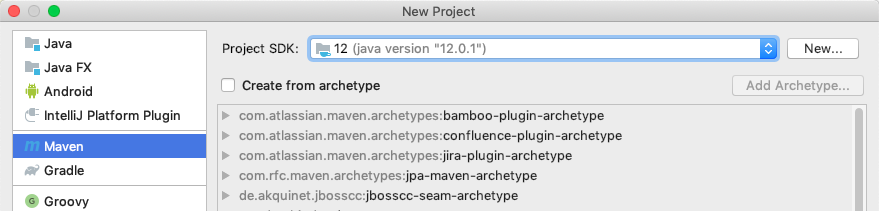
\includegraphics[scale=0.46]{image/5.png}
\end{figure}

打开 IntelliJ 的偏好设置,定位到 Java Compiler ,将 WebAccessLog 的 Target Bytecode Version 设置为与 JDK 版本号相同的版本。

\begin{figure}[!ht]
\centering
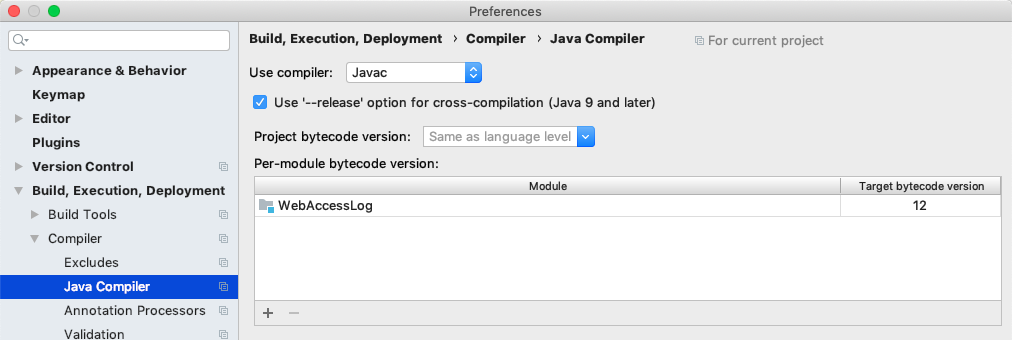
\includegraphics[scale=0.4]{image/6.png}
\end{figure}

\subsection{配置依赖}

新建项目后,编辑 Maven 配置文件 pom.xml 。

\subsubsection{添加源}

在 project 内尾部添加

\begin{lstlisting}
<repositories>
    <repository>
        <id>apache</id>
        <url>http://maven.apache.org</url>
    </repository>
</repositories>
\end{lstlisting}

\subsubsection{添加依赖}

我们只需要用到基础依赖 hadoop-core 和 hadoop-common 。

在 project 内尾部添加

\begin{lstlisting}
<dependencies>
    <dependency>
        <groupId>org.apache.hadoop</groupId>
        <artifactId>hadoop-core</artifactId>
        <version>1.2.1</version>
    </dependency>
    <dependency>
        <groupId>org.apache.hadoop</groupId>
        <artifactId>hadoop-common</artifactId>
        <version>2.7.2</version>
    </dependency>
</dependencies>
\end{lstlisting}

对于 hadoop-core 和 hadoop-common 的版本号,我们建议在 Google 搜一个最新的填上去。

修改 pom.xml 完成后,IntelliJ 会提示 Maven projects need to be Imported ,点击 Import Changes 以更新依赖。

\subsection{主程序}

在 src $rightarrow$ main $rightarrow$ java 下新建一个 WebAccessLog 类,在里面写 MapReduce 程序。

\subsection{配置输入文件}

我的 WebAccessLog 程序读取每行访问信息,然后统计相关统计量。首先在 WebAccessLog 目录下(src 同级目录)新建一个文件夹 input ,并添加一个或多个文本文件到 input 中。

\subsection{配置运行参数}

这里我们需要配置此程序运行时的 Main class ,以及 WebAccessLog 需要的输入输出路径。

在 IntelliJ 菜单栏中选择 Run $\rightarrow$ Edit Configurations ,在弹出来的对话框中点击 $+$ ,新建一个 Application 配置。配置 Main class 为 WebAccessLog,Program arguments 为 input/ output/ ,即输入路径 input 文件夹,输出为 output 。

\begin{figure}[!ht]
\centering
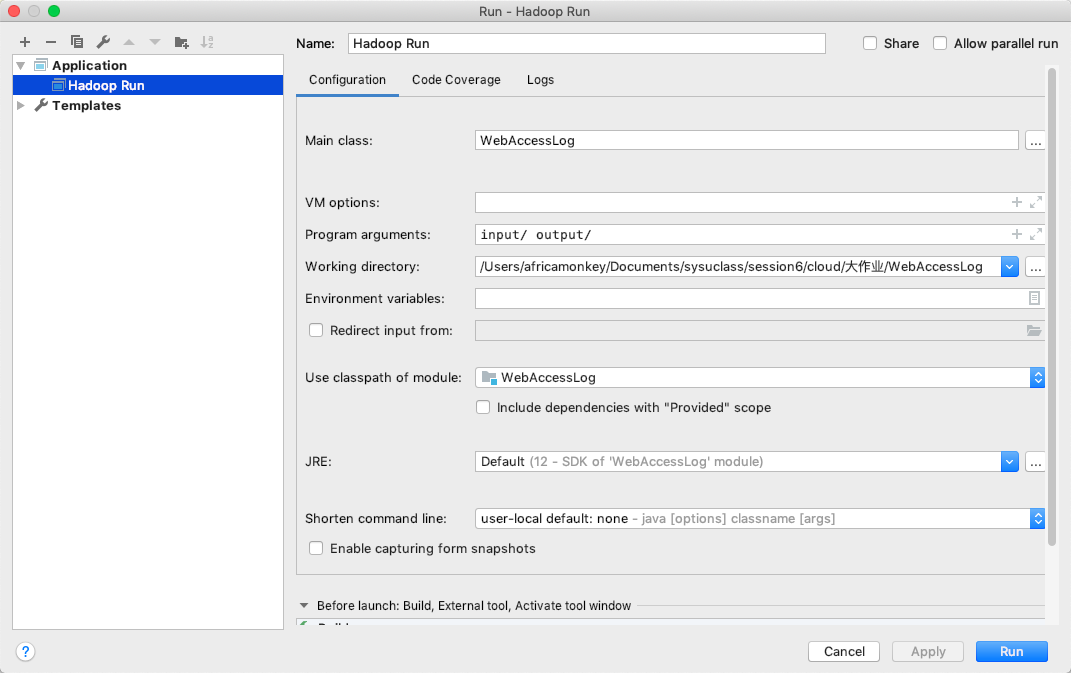
\includegraphics[scale=0.4]{image/7.png}
\end{figure}

\newpage

\subsection{运行}

点击菜单栏 Run $\rightarrow$ Run 'WebAccessLog' 即开始运行 MapReduce 程序,IntelliJ 下方会显示 Hadoop 的运行输出。程序运行完毕后,IntelliJ 左上方会出现新的文件夹 output ,其中的 part-r-00000 就是运行的结果。

\subsection{运行结果}

从实验开始,到撰写本报告为止, Apache 日志记录了 $3$ 天共 $25925$ 次请求。

\subsubsection{统计每天的请求数、数据量}

\begin{figure}[!ht]
\centering
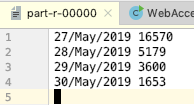
\includegraphics[scale=0.5]{image/10.png}
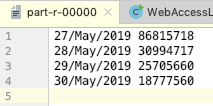
\includegraphics[scale=0.5]{image/11.png}
\end{figure}

其中,左图表示的是请求数,右图表示的是数据量(字节)。可以看到请求数和数据量是呈正相关的。

你们可能会觉得很奇怪,访问量为什么会指数级地减少。其原因是 $28$ 号为提交作业的 DDL 。过了 DDL ,又没有新的作业布置下来,自然访问量就少了。

通过分析这个数据,我们可以很轻松地分析出老师布置作业的时间和频率。

\newpage

\subsubsection{统计每个时段的请求数、数据量}

\begin{figure}[!ht]
\centering
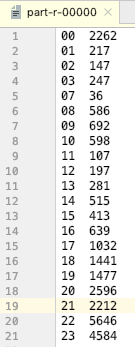
\includegraphics[scale=0.5]{image/8.png}
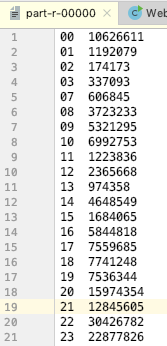
\includegraphics[scale=0.5]{image/9.png}
\end{figure}

我们能看出来,从 $20$ 点至次日 $1$ 点是网站访问的高峰,在 $22$ 点至 $23$ 点达到峰值。看来我们的同学们喜欢在晚上做题,甚至有同学在凌晨 $1$ 点至 $4$ 点做题……我都快惊呆了!

\subsubsection{统计每个 IP 地址的请求数、数据量}

\begin{figure}[!ht]
\centering
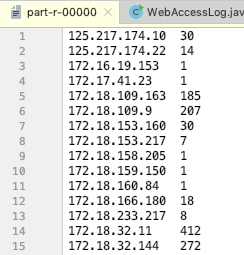
\includegraphics[scale=0.5]{image/12.png}
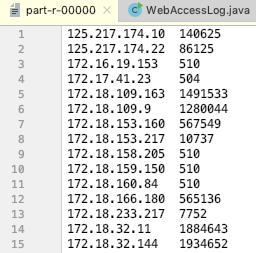
\includegraphics[scale=0.5]{image/13.png}
\end{figure}

我们可以对每个 IP 地址统计它的请求数和数据量,若某个 IP 地址产生的数据量远超过上传下载作业所需的作业量,我们就能把这样的 IP 地址找出来,并对这个 IP 所产生的数据做进一步的调查与分析。

\section{分布式运行}

\subsection{Master 服务器的搭建}

为实现分布式运行,我先在阿里云部署 $1$ 台服务器作为 Master ,待安装好全套 Hadoop 环境和 JDK 环境后,用 Master 制作镜像,然后使用 Master 镜像再在阿里云申请 $3$ 台服务器作为 Slave 。

硬件配置
\begin{itemize}
\item CPU: Intel(R) Xeon(R) Platinum 8163 CPU @ 2.50GHz ;核心数: $1$ ;平均基准 CPU 计算性能: $10\%$
\item RAM: 1 GB
\item 内网带宽: 200 Mbps
\end{itemize}

服务器操作系统: Ubuntu 18.04 LTS

为方便起见,在本实验中使用的用户均为 root 。

\subsection{Hadoop 环境配置}

\subsubsection{下载 Hadoop}

访问 Apache 网站获取下载链接,在 Master 上直连 Apache 官网下载。下载完成后解压到当前目录下。

在 root 的用户目录 `/root/' 下执行:

\begin{lstlisting}[language=bash]
wget https://www-us.apache.org/dist/hadoop/common/hadoop-3.1.2/hadoop-3.1.2.tar.gz
tar -zxvf hadoop-3.1.2.tar.gz
\end{lstlisting}

\subsubsection{下载和安装 JDK}

在 root 的用户目录 `/root/' 下执行:

\begin{lstlisting}[language=bash]
wget --no-check-certificate -c --header "Cookie: oraclelicense=accept-securebackup-cookie"  https://download.oracle.com/otn-pub/java/jdk/12.0.1+12/69cfe15208a647278a19ef0990eea691/jdk-12.0.1_linux-x64_bin.deb
dpkg -i jdk-12.0.1_linux-x64_bin.deb
\end{lstlisting}

\subsubsection{设置 HDFS 服务器地址}

在 `/root/hadoop-3.1.2/etc/hadoop/core-site.xml' 中:将 localhost 改为 Master 服务器的 IP 地址。

\begin{lstlisting}
<configuration>
    <property>
        <name>fs.defaultFS</name>
        <value>hdfs://localhost:9000</value>
    </property>
</configuration>
\end{lstlisting}

\subsubsection{设置环境变量}

在 `/root/.bashrc' 文件尾追加:

\begin{lstlisting}[language=bash]
export ROOT="root"
export HDFS_NAMENODE_USER=$ROOT
export HDFS_DATANODE_USER=$ROOT
export HDFS_SECONDARYNAMENODE_USER=$ROOT
export YARN_RESOURCEMANAGER_USER=$ROOT
export YARN_NODEMANAGER_USER=$ROOT
export JAVA_HOME="/usr/lib/jvm/jdk-12.0.1"
export JRE_HOME="${JAVA_HOME}/jre"
export HADOOP_HOME="/root/hadoop-3.1.2"
export CLASSPATH=".:${JAVA_HOME}/lib:${JRE_HOME}/lib:$($HADOOP_HOME/bin/hadoop classpath)"
export PATH="${JAVA_HOME}/bin:$PATH"
export HADOOP_COMMON_LIB_NATIVE_DIR=$HADOOP_HOME/lib/native
export HADOOP_OPTS="-Djava.library.path=$HADOOP_HOME/lib"
\end{lstlisting}

\subsubsection{单机试运行示例程序}

在 `/root/hadoop-3.1.2' 中运行:

\begin{lstlisting}[language=bash]
bin/hadoop jar share/hadoop/mapreduce/hadoop-mapreduce-examples-3.1.2.jar grep input output 'dfs[a-z.]+'
\end{lstlisting}

\subsubsection{配置 SSH 免密登录}

首先生成一组公钥和私钥

\begin{lstlisting}[language=bash]
ssh-keygen -t rsa -P '' -f ~/.ssh/id_rsa
\end{lstlisting}

将该公钥列入本机白名单,凭该公钥对应的私钥可登录本机。

\begin{lstlisting}[language=bash]
cat ~/.ssh/id_rsa.pub >> ~/.ssh/authorized_keys
\end{lstlisting}

\subsection{创建及配置 Slave 服务器}

我们将 Master 服务器创建镜像,然后使用该镜像创建 $3$ 台 Slave 服务器。由于我们已经在镜像中配置好 Hadoop 、JDK 、环境变量和免密登录,我们在 Slave 机器上无需作任何配置,只需保证服务器正常运行即可。

我们需记录下阿里云为 Slave 服务器分配的 IP 地址(如不喜欢可更改)。

\begin{figure}[!ht]
\centering
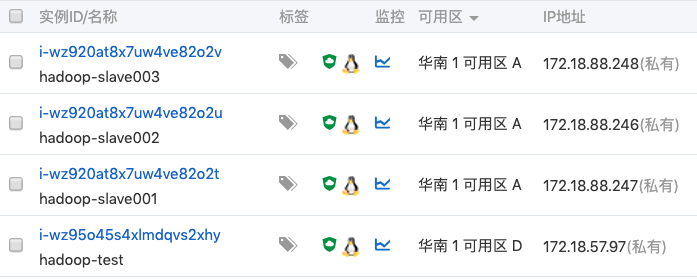
\includegraphics[scale=0.5]{image/14.png}
\end{figure}

为方便管理,我们在 Master 服务器上的 /etc/hosts 文件中添加 $3$ 台 Slave 服务器的别名。

\begin{figure}[!ht]
\centering
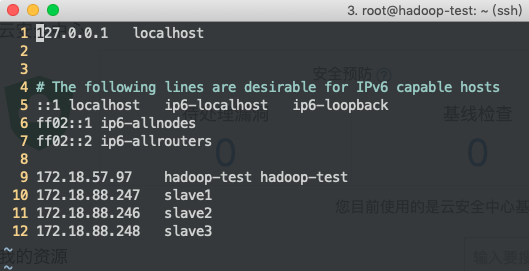
\includegraphics[scale=0.5]{image/15.png}
\end{figure}

\subsection{在 Master 服务器上加入 Slave 服务器}

在 `/root/hadoop-3.1.2/etc/hadoop/workers' 中,加入 Slave 服务器的IP 地址、别名或域名。

\begin{lstlisting}
slave1
slave2
slave3
\end{lstlisting}

\subsection{自动初始化和自动运行脚本}

每次初始化集群都要敲一大堆命令,由于我非常懒,不想次次都敲,就写了个脚本。代码的意思是,先停止 Hadoop  的全部服务,把该清的清了,创建并格式化 HDFS ,再启动所有服务,最后在 HDFS 下为 root 用户创建一个用户目录。

初始化脚本 `/root/hadoop-3.1.2/init.sh' :

\begin{lstlisting}[language=bash]
sbin/stop-all.sh
ssh localhost "rm -rf /tmp/*"
ssh slave1 "rm -rf /tmp/*"
ssh slave2 "rm -rf /tmp/*"
ssh slave3 "rm -rf /tmp/*"
bin/hdfs namenode -format
sbin/start-all.sh
bin/hdfs dfs -mkdir /user
bin/hdfs dfs -mkdir /user/root
\end{lstlisting}

每次启动之前要将 HDFS 上的 input 、output 文件夹删除,然后将本地的 input 文件夹上传至 HDFS 。为此,我也写了个启动脚本。

启动脚本 `/root/hadoop-3.1.2/start\_task.sh' :

\begin{lstlisting}[language=bash]
bin/hdfs dfs -rm -r output/
bin/hdfs dfs -rm -r input/
bin/hdfs dfs -put input/
bin/hadoop jar ~/WebAccessLog/WebAccessLog.jar WebAccessLog input output
\end{lstlisting}

\subsection{运行}

执行初始化脚本,打开浏览器,访问 http://Master-ip:9870 ,可以看到 Hadoop 集群的运行状态

\begin{figure}[!ht]
\centering
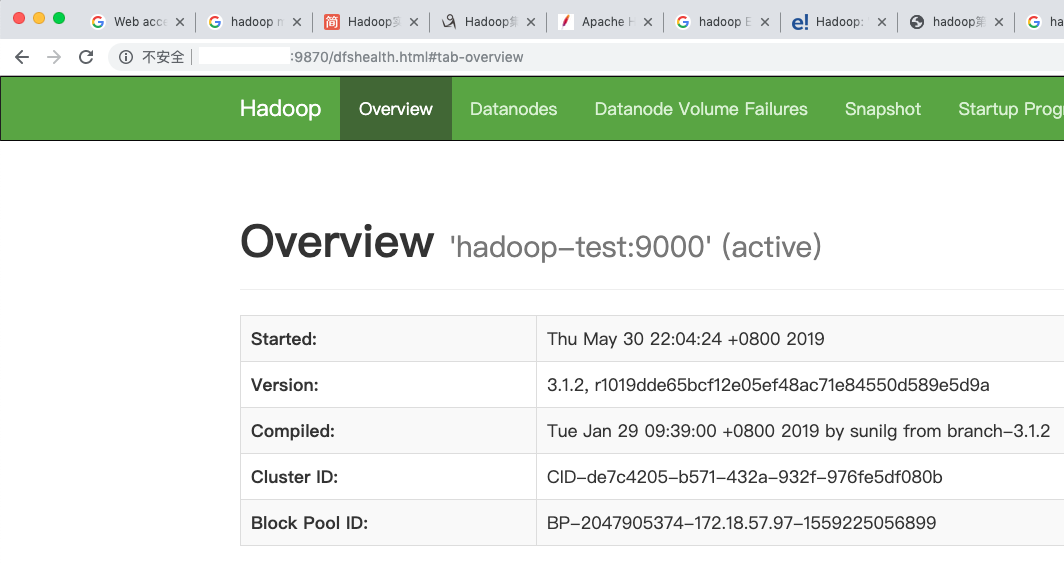
\includegraphics[scale=0.35]{image/16.png}
\end{figure}

\newpage 

\begin{figure}[!ht]
\centering
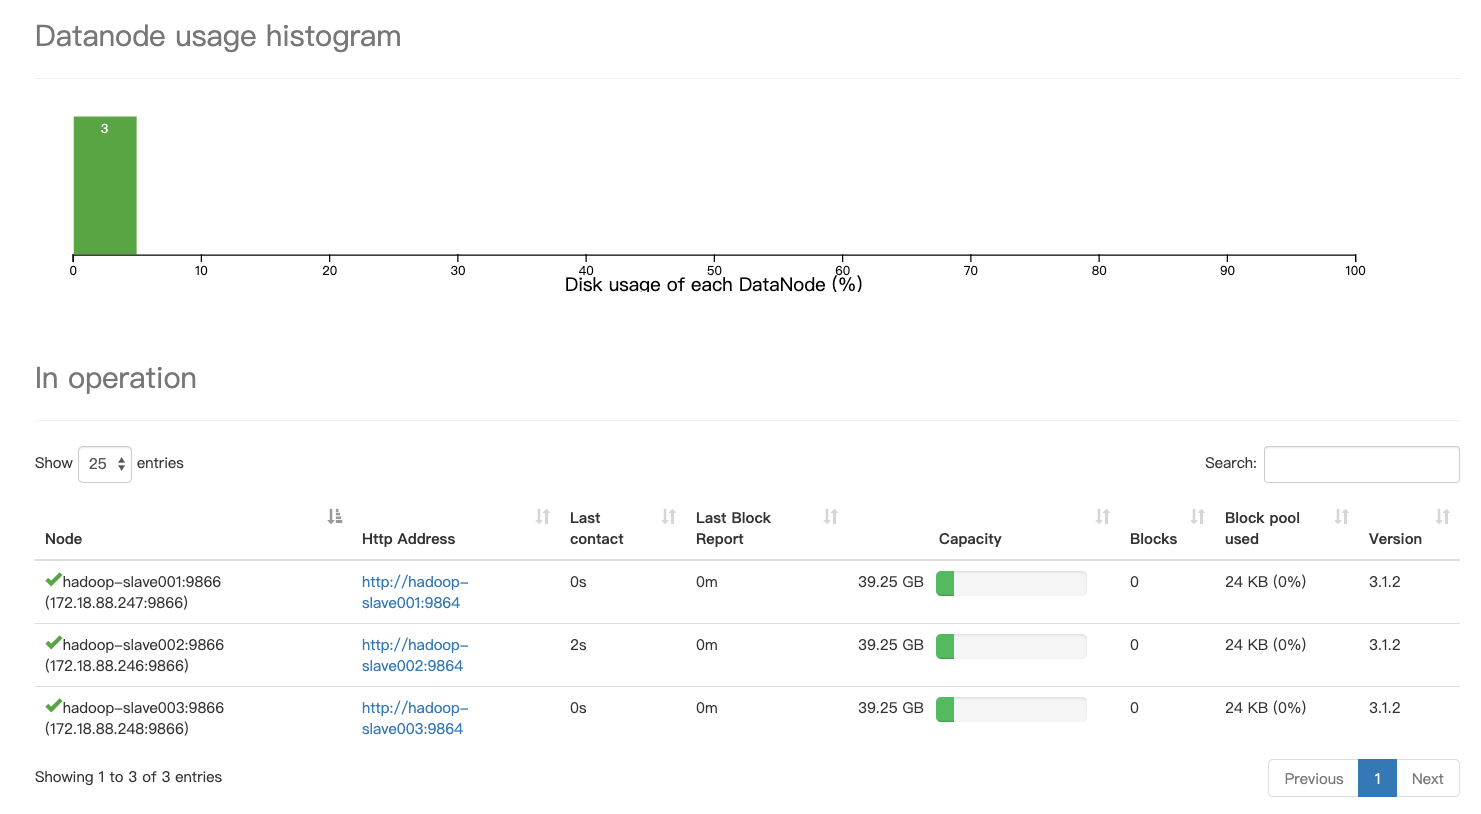
\includegraphics[scale=0.3]{image/3.png}
\end{figure}

除了在网页能查看,我们还可以通过在 Master 上执行 bin/hdfs dfsadmin -report 在命令行查看 Hadoop 集群的运行状态。

\begin{figure}[!ht]
\centering
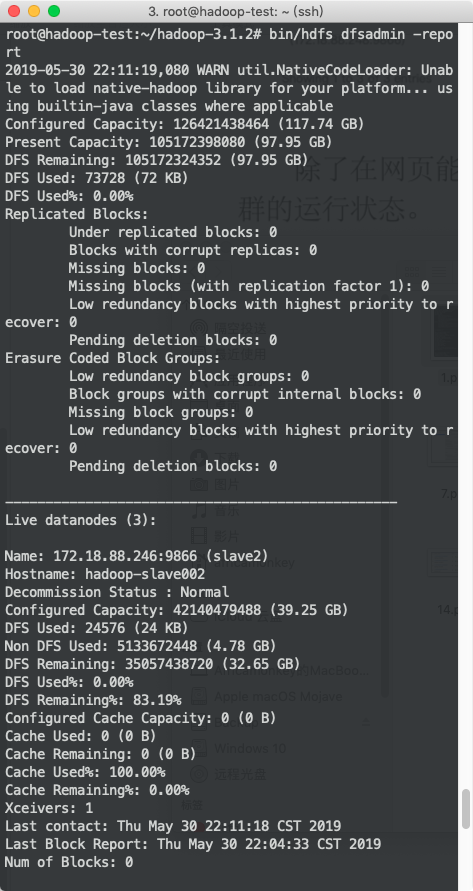
\includegraphics[scale=0.38]{image/1.png}
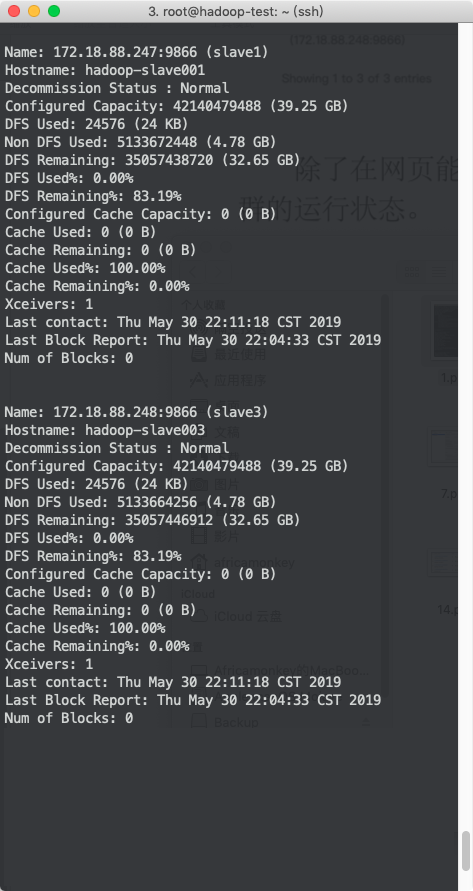
\includegraphics[scale=0.38]{image/2.png}
\end{figure}

上传 WebAccessLog.java 到 Master 服务器上,放在 `/root/WebAccessLog/' 下。

编译 WebAccessLog.java :

\begin{lstlisting}[language=bash]
javac WebAccessLog.java
\end{lstlisting}

将生成的 class 打包:

\begin{lstlisting}[language=bash]
jar -cvf WebAccessLog.jar *.class
\end{lstlisting}

上传 access.log 日志到 `/root/hadoop-3.1.2/input/' 下。

然后执行启动脚本,期间会有 mapreduce 的过程日志刷屏。

\begin{lstlisting}[language=bash]
./start_task.sh
\end{lstlisting}

查看结果:

\begin{lstlisting}[language=bash]
bin/hdfs dfs -cat output/*
\end{lstlisting}

下载结果:

\begin{lstlisting}[language=bash]
bin/hdfs dfs -get output
\end{lstlisting}

\subsection{性能测试}

由于我们没有这么多数据,我们将这 $27002$ 条(与前面的数字不同,原因是撰写报告的时候又多了一些访问量)的数据复制 $200$ 份,这样大约产生 $540$ 万条数据。我们就用这些数据来测试 Hadoop 性能。

我们以“统计每个 IP 地址的数据量”的程序为例,分别测试在 $1$ 个、 $2$ 个和 $3$ 个 Slave 的条件下,完成 MapReduce 所需的时间。

\begin{table}[!ht]
\centering
\begin{tabular}{|l|l|}
\hline
Slave 数量 & 用时 \\
\hline
1 & 90.037s \\
\hline
2 & 91.052s \\
\hline
3 & 90.552s \\
\hline
\end{tabular}
\end{table}

咦这就奇怪了,为什么无论是几台 Slave ,完成 MapReduce 的时间都是 90s 左右呢?

我发现我选服务器选的是最便宜的入门级(共享)……很大可能它们 $3$ 个 Slave 都是共享同一个核心的 CPU 跑的。

然后我开了 $3$ 台配置好一点的机器,测得耗时分别是 95.319s 、94.669s 、93.411s ,原因应该不是我之前的猜测。

我在服务器跑的过程中监控了 CPU 使用率(如下图),发现只有 Master 的 CPU 使用率是比较高的,而 Slave 的使用率都比较低。我认为 Slave 只运行了 HDFS ,而未实际参与 Map/Reduce 的计算,那这个 Slave 就很没用了。

\begin{figure}[!ht]
\centering
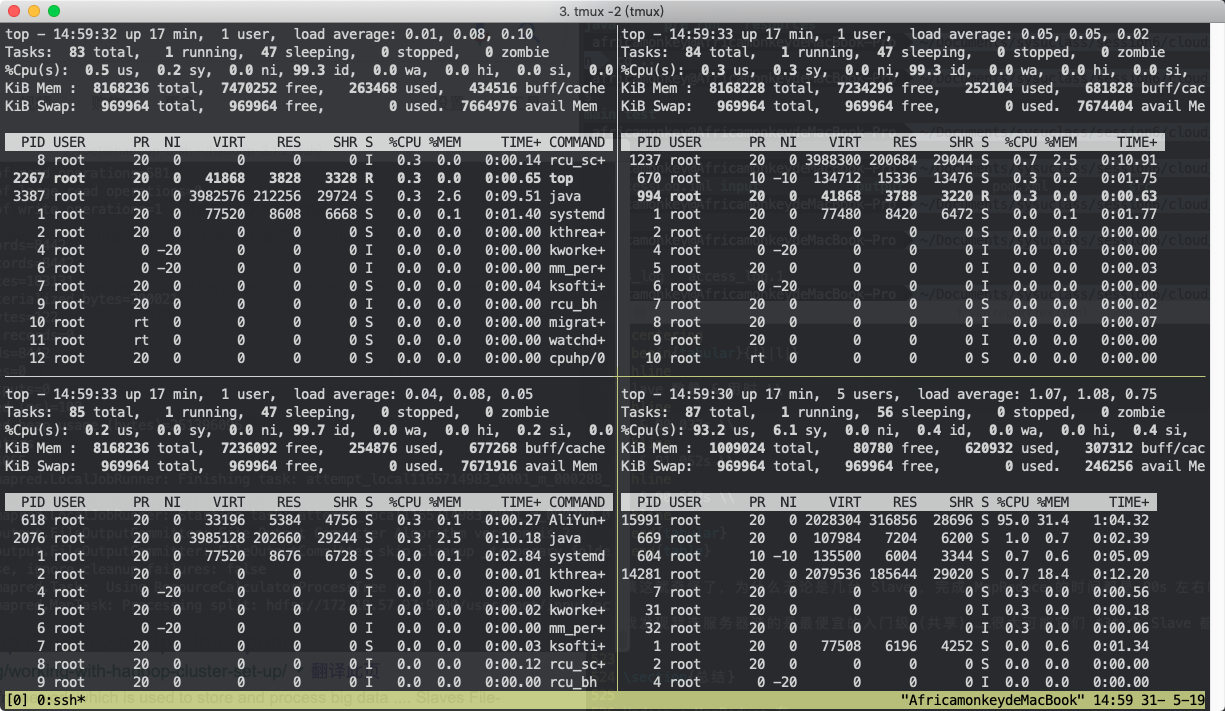
\includegraphics[scale=0.35]{image/18.png}
\end{figure}

\section{总结}

MapReduce 还是处理大数据的很有用的工具,它能帮助我们对访问记录等做统计数据的工作。在本问题中, MapReduce 切切实实地帮助我们分析了日访问量、用户活跃时间、可疑 IP 地址行为,并可根据实际需要添加 HTTP 状态码分析、扩展名分析等功能。加入这些功能后,可以通过 HTTP 状态码查找出遇到问题的网页,也可以帮助我们统计静态资源使用量,从而更精确地把某些静态资源移到 CDN 上。 Hadoop 使用 Java 语言,使得 MapReduce 还能跨平台工作,甚至是将源代码编译后可直接在别的服务器上运行。Hadoop 的配置不复杂,但没能充分利用 Slave 服务器的 CPU 资源。

用 Hadoop 还有个好处就是文档丰富,用户也比较多,所以在搜索引擎中搜索一个问题总是大概率能找到答案。用 Java 写陌生的继承类必须要有 IDE 。我在 Android 中使用了 Android Studio ,觉得非常棒,可以很清晰地看到继承类的定义、方法的定义等等;另外,它在程序运行前、运行后都可以添加脚本,方便自动化配置输入输出文件运行。我查看“关于”知 Android Studio 是在 IntelliJ 平台开发的。于是我在 JetBrain 官网找是否有 Java 的 IDE ,那当然是有的啦——IntelliJ IDEA 。IntelliJ IDEA 的界面、布局、快捷键跟 Android Studio 都极为相似,基本上是零学习成本上手。

\end{document}
